% !Mode:: "TeX:UTF-8"

\chapter{面向花朵位姿检测的目标分割}\label{ch:3}
\iffalse
\section{引言}
在现代农业中,自动化授粉技术正在成为解决劳动力短缺、提高作物产量和品质的重要手段。其中,机械臂柔顺控制的精准授粉任务对环境感知能力提出了极高的要求。要实现高效、稳定的授粉操作,机械臂需要能够准确感知花朵的空间特征,包括位置、形态、朝向等信息。这些信息的准确性直接决定了授粉的成功率和稳定性,因此,位姿检测是精准授粉技术的关键环节。

为了感知环境信息,机器人通常依赖各种传感器,例如RGB摄像头、深度相机、激光雷达等。其中,RGB-D深度相机由于能够同时提供彩色信息和深度信息,且成本较低,成为农业领域常用的视觉传感器。然而,在复杂的温室或田间环境中,由于光照条件的变化、花朵表面反射特性、叶片遮挡等因素,深度相机采集的数据往往存在噪声、空洞、误差等问题,导致位姿检测精度下降。因此,在使用深度相机数据进行位姿估计前,必须对其进行预处理,包括深度数据修正、去噪、补全等,以确保位姿信息的准确性。

此外,为了便于人机交互和授粉轨迹规划,本章提出了一种基于对称空间的花朵位姿检测方法,能够实时构建虚拟空间并同步更新授粉目标花朵的三维位置和朝向信息。该方法可以计算空间中花朵的位姿,为机械臂的授粉任务提供直观、准确的位姿参考信息,并为后续优化机械臂的运动轨迹提供数据。本章方法的整体技术路线主要包括目标分割、深度校正和位姿估计三个部分:首先,使用基于深度学习的实例分割方法对花朵区域进行精确提取;其次,采用深度校正算法对RGB-D相机采集的数据进行优化,以减少噪声并提高深度信息的可靠性;最后,结合三维重建技术,估计花朵的位姿信息。
\fi
\section{引言}

在机械臂执行精准授粉任务的过程中,准确识别花朵的位置和形态是确保授粉成功的关键。然而,在实际的农业场景中,花朵通常处于复杂的背景环境中,容易受到光照变化、遮挡以及花朵自身形态变化的影响,导致分割难度大幅增加。因此,如何高效、准确地分割花朵区域,成为花朵位姿检测中的核心问题。传统的图像处理方法,例如基于颜色分割、边缘检测或形态学处理的手工特征提取方法,虽然在特定条件下能够取得一定的分割效果,但面对不同品种的花朵、复杂的光照环境以及动态变化的遮挡情况,其鲁棒性较差,难以满足自动化授粉系统的要求。

为了克服这些挑战,本章采用基于深度学习的目标分割方法,通过训练神经网络模型,使其能够自动提取花朵的特征并实现高精度分割。在深度学习的发展中,实例分割技术已经成为解决目标分割问题的主流方法,其中 Mask-RCNN 和 YOLACT 作为两种代表性模型,分别适用于高精度分割和高实时性分割的任务。在本章的研究中,我们结合两者的优势,根据不同应用场景选择合适的目标分割方法,以确保花朵分割的准确性和实时性兼顾。

\section{方法}
\subsection{Mask-RCNN}
 \begin{figure}[htb]
	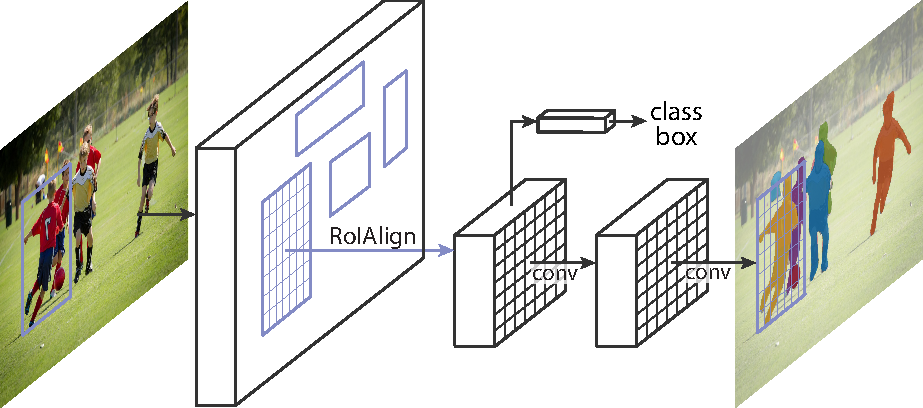
\includegraphics[width=0.6 \textwidth]{mask-rcnn}
	\caption[实例分割Mask-RCNN 框架]{实例分割Mask-RCNN 框架} % 中括号中内容为插图索引中显示内容,可在题注内容过长时使用
	\label{fig:mask-rcnn}
\end{figure}
Mask-RCNN是一种经典的实例分割模型,它是在 Faster-RCNN 目标检测框架的基础上增加了掩膜分割(Mask)分支,使其不仅能够检测目标,还能在像素级别进行分割,如\cref{fig:mask-rcnn}所示。这一特性使得 Mask-RCNN 在花朵检测中具有较高的精度,能够精准地分割出花朵区域,而不受背景影响。在 Mask-RCNN 的模型结构中,首先采用 ResNet-50 或 ResNet-101 作为主干网络,通过卷积神经网络提取图像的高层次特征,并结合特征金字塔网络(FPN, Feature Pyramid Network),增强对不同尺度花朵的检测能力。随后,区域候选网络(RPN, Region Proposal Network)生成候选目标区域,并通过非极大值抑制(NMS, Non-Maximum Suppression)去除冗余的候选框,确保检测的可靠性。最后,ROIAlign 机制用于对目标区域进行精确的特征提取,并通过一个全卷积网络(FCN, Fully Convolutional Network)生成目标的掩膜,实现高精度的实例分割。

Mask-RCNN 在花朵目标分割中的应用表现优异,能够有效应对复杂背景和遮挡问题。然而,由于该模型采用了串行的目标检测和实例分割流程,在计算上开销较大,推理速度相对较慢。在实验环境(NVIDIA GTX 1080 Ti)下,其分割速度约为 5FPS,难以满足实时授粉任务的需求。因此,在实际应用中,若对计算速度要求较高,需要寻找更高效的分割方法,以满足农业机械臂在自动化授粉中的实时性需求。

\subsection{YOLACT}
 \begin{figure}[htb]
	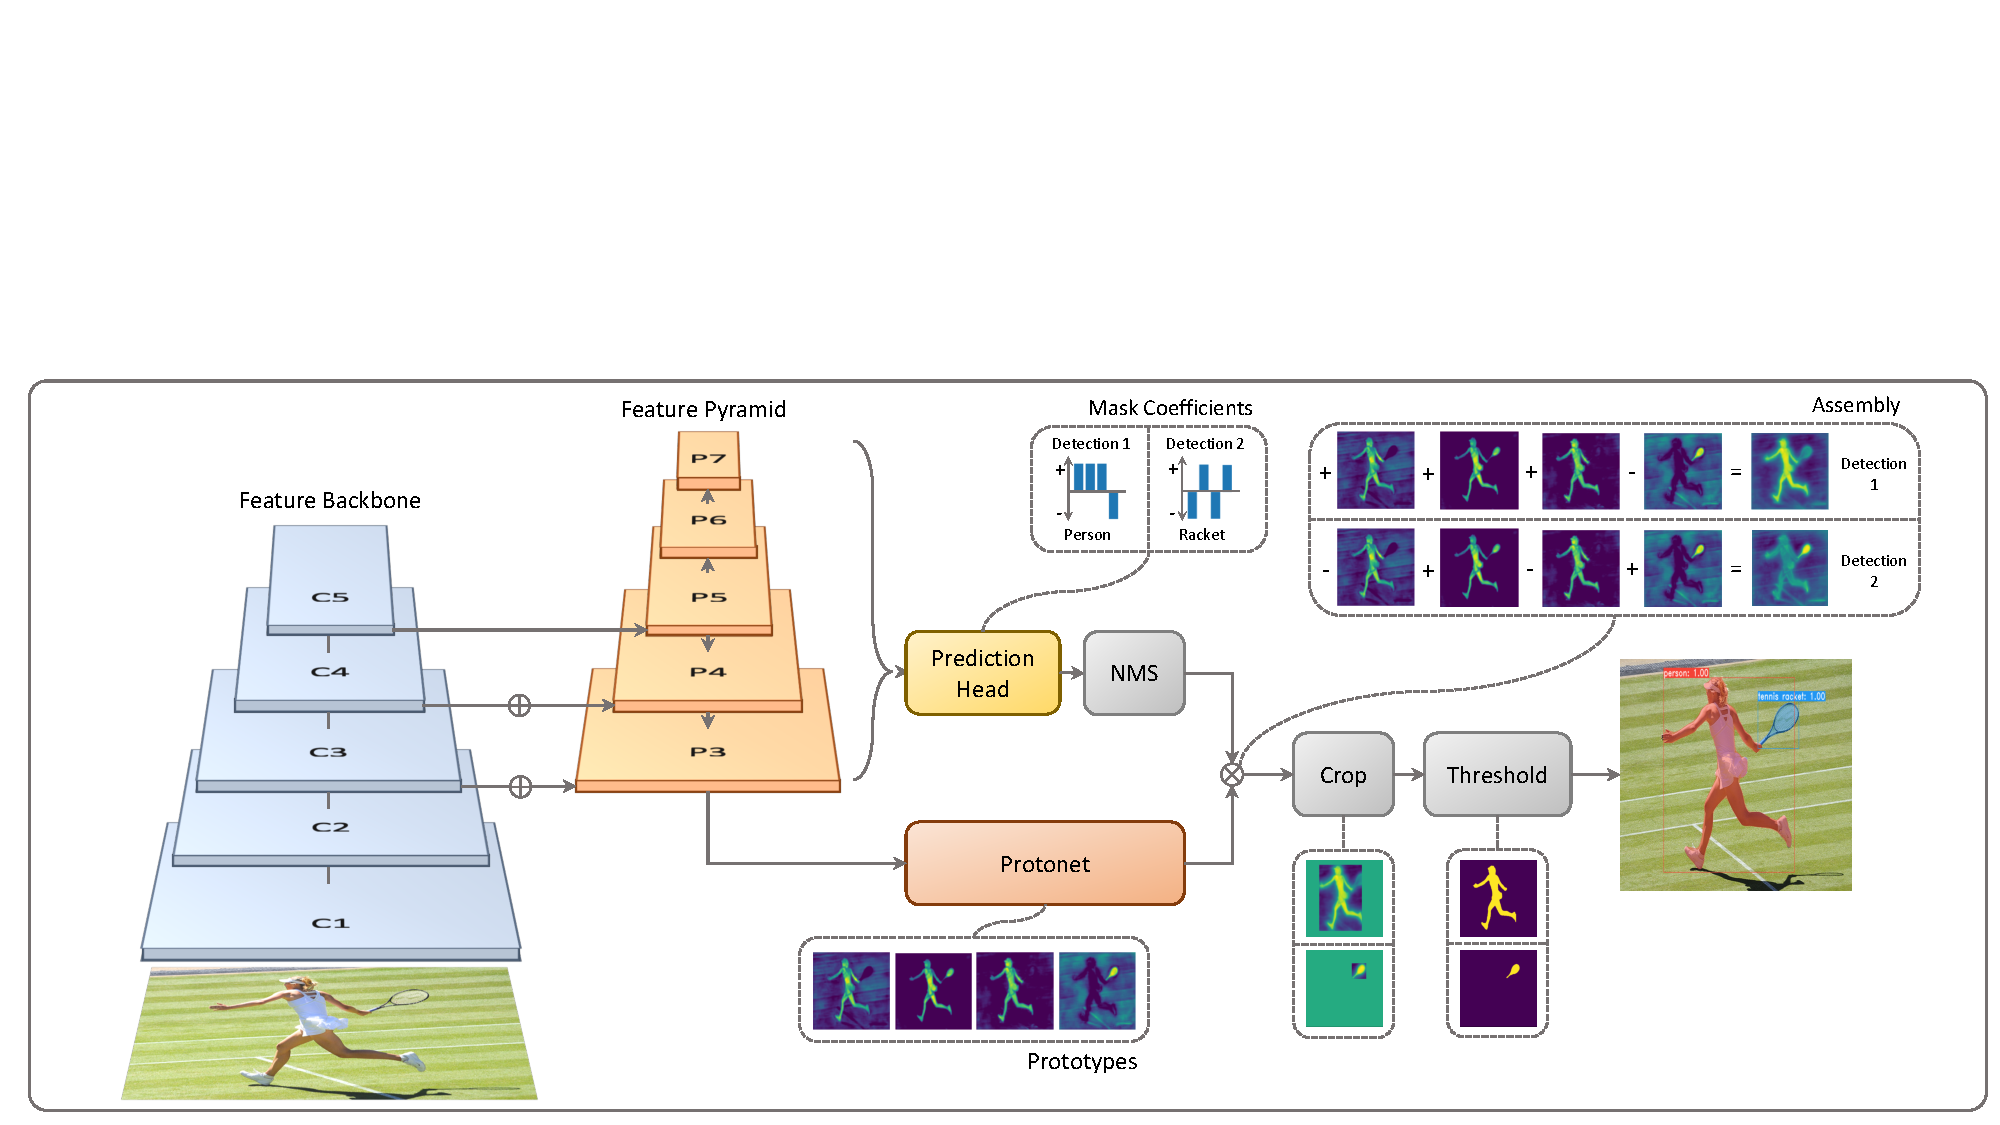
\includegraphics[width=0.8 \textwidth]{yolact}
	\caption[yolact模型架构图]{yolact模型架构图} % 中括号中内容为插图索引中显示内容,可在题注内容过长时使用
	\label{fig:yolact}
\end{figure}
为了解决 Mask-RCNN 在推理速度上的不足,本章引入了 YOLACT(You Only Look At Coefficients, Bolya et al., 2019) 作为优化方案。YOLACT 的核心优势在于 并行执行目标检测和图像分割,避免了 Mask-RCNN 先检测再分割的串行结构,从而大幅提升计算效率。在 YOLACT 的架构中,如\cref{fig:yolact}所示,仍然采用 ResNet-50 或 ResNet-101 作为主干网络,并结合 FPN 提取多尺度特征。在目标检测方面,YOLACT 采用单阶段检测框架,使其可以直接对目标进行分类和定位,而不需要额外的候选区域生成过程。此外,其分割分支通过一个专门的掩膜预测网络,能够在检测的同时进行掩膜预测,使得整个推理过程更加高效。

YOLACT 在授粉任务中的应用主要体现在其优异的实时性。相比于 Mask-RCNN,其计算复杂度大幅降低,在相同实验环境下推理速度可达 34FPS,远高于 Mask-RCNN 的 5FPS。这种高效的计算能力使其更加适用于实时授粉任务,尤其是在需要快速识别和分割花朵,以指导机械臂进行柔顺控制的应用场景。然而,YOLACT 在分割精度上相较于 Mask-RCNN 略有下降,尤其是在边缘处理方面可能存在一定的误差。因此,在高精度需求的场景(如授粉过程中需要确保机械臂末端精准对准花蕊)时,Mask-RCNN 依然是更优的选择,而在需要实时响应的场景(如大规模花卉授粉)中,YOLACT 则更加合适


\section{实验设计与结果分析}
\subsection{实验环境}
本章实验的软硬件设备如表下所示:
\begin{table}[htbp]
	\caption[目标分割实验环境]{目标分割实验环境}
	\setlength{\tabcolsep}{14mm}{ % 因表格过窄,手动设置宽度为7mm
		\begin{tabular}{clc}
			\toprule
			序号    &  设备    & 型号   \\
			\midrule
			1 & realsence相机  & D435i     \\
			2 & cpu  & intelCorei5-13600     \\
			3 & 内存 & 32GB   \\
			4 & 操作系统  & window10    \\
			5 & 显卡     & NVIDIA GeForce GTX3090 \\
			6 & 编译语言    & python3.8       \\
			7 & 深度学习框架    & Pytorch2.4       \\
			\bottomrule
	\end{tabular}}
	\label{tab:division-of-microchannels}
\end{table}
\subsection{数据集} 


 \begin{figure}[htb]
	\includegraphics[width=0.8 \textwidth]{folower.png}
	\caption[部分数据集图片]{部分数据集图片} % 中括号中内容为插图索引中显示内容,可在题注内容过长时使用
	\label{fig:folower.drawio}
\end{figure}
在本研究中,为了构建一个高质量的目标实例分割数据集,我们在实验大棚内进行了大规模的数据采集,采集的数据如\cref{fig:folower.drawio}所示。实验大棚的环境与真实农业应用场景相似,包括自然光照、人工补光、叶片遮挡等多种复杂因素,这些因素都会影响机械臂授粉时的视觉感知能力。因此,我们在数据采集过程中特别关注不同光照条件和不同视角的花朵图像,以确保数据集能够涵盖各种可能遇到的场景,提高分割模型的泛化能力。

数据采集采用了一种滑动拍摄的方式,即让RGB-D 深度相机固定在机械臂上,并以恒定速度沿着花朵区域移动,同时在不同角度和光照条件下进行连续拍摄。机械臂的移动轨迹覆盖了花朵的不同高度、朝向,并在多个点位停留进行固定拍摄,以获取完整的花朵视角信息。相比于静态拍摄,滑动拍摄的方式能够更全面地记录花朵在机械臂运动过程中不同视角下的外观变化,使得数据更符合实际应用需求。此外,考虑到授粉任务可能发生在不同时间段,我们分别在上午、正午和下午三个时段进行了数据采集,以涵盖不同的光照条件。



在数据采集过程中,我们使用了realsence相机,并将其安装在UR5机械臂末端,使其能够随机械臂的运动采集到稳定的图像和深度信息。相机的分辨率设置为 1920×1080(RGB) ,并采用自动曝光,以适应不同的光照环境。在拍摄过程中,相机的采集频率设定为每 0.5 秒拍摄一张图像,每个角度平均获取10 张图像,确保数据的多样性和完整性。
\begin{table}[htbp]
	\caption[不同光照条件数据采集]{不同光照条件数据采集}
	\setlength{\tabcolsep}{14mm}{ % 因表格过窄,手动设置宽度为7mm
		\begin{tabular}{clc}
			\toprule
			光照条件    &  采集张数    & 占比 (\%)  \\
			\midrule
			正常环境 & 420  & 37.8 \\
			强光环境 & 238  & 21.4    \\
			阴影环境 & 210 & 19.0   \\
			背光环境 & 242  & 21.8    \\
			总计 & 1110 & 100 \\
			\bottomrule
	\end{tabular}}
	\label{tab:dataset}
\end{table}

经过多次实验和数据收集,我们最终获得了 1110 多张 RGB 图像,并同时存储了其对应的深度图像,采集的数据详细如\cref{tab:dataset}所示。这些数据不仅涵盖了花朵在不同光照、角度下的外观变化,同时也包含了一些叶片遮挡、强光反射、阴影影响等特殊场景,这些额外的因素有助于训练一个更加鲁棒的目标分割模型。为了确保数据质量,我们对数据进行了筛选,去除了模糊、过曝或不完整的图像,并对数据集的类别分布进行了统计分析。

在数据标注过程中以人工标注的方式标注,我们将标注结果存储为 JSON 格式,包括目标类别、掩膜坐标信息,以及对应的 RGB 图像和深度图像,以便后续用于深度学习模型的训练和测试。

\subsection{实验设计} 
本实验的主要目的是评估基于深度学习的目标分割方法在花朵位姿检测任务中的表现,并验证 Mask-RCNN 和 YOLACT 在不同场景下的分割精度、计算效率以及对复杂环境(如光照变化、遮挡情况等)的适应性。重点关注模型的分割精度、计算效率以及在复杂场景中的适应性。通过对比不同分割模型的性能,确定在自动化授粉任务中最适合的目标分割方法。

在实验方法上,我们采用了相同的训练和测试环境,以保证不同分割模型的可比性。实验在NVIDIA RTX 3090 GPU 上运行,使用 PyTorch2.4 作为深度学习框架。对于 Mask-RCNN,我们选择 ResNet-101 作为主干网络,并结合 FPN(Feature Pyramid Network) 以提高对不同尺度花朵的检测能力。YOLACT 采用了ResNet-50 作为主干网络,同样结合 FPN 进行特征提取。为了优化训练过程,我们使用COCO预训练模型进行参数初始化,并在实验大棚数据集上进行50轮微调训练。训练过程中,批量大小设定为 8,学习率初始值为 0.001,并在训练过程中进行数据增强,包括随机裁剪、水平翻转、颜色扰动等,以提升模型的泛化能力。

在实验指标的选择上,我们设定了三个衡量标准。首先,mIoU(mean Intersection over Union)作为分割精度的重要指标,用于衡量模型预测掩膜与真实标注掩膜的重叠程度,mIoU 越高,说明模型分割出的目标区域越精准。除了分割精度,我们还考虑了计算效率(FPS, Frames Per Second),即模型每秒可以处理的帧数,这对于实时授粉任务尤为关键,FPS 值越高,说明模型的推理速度越快。此外,为了测试模型的鲁棒性,我们设计了多种复杂场景,包括光照变化、部分遮挡和严重遮挡等环境,并观察 mIoU 在这些环境下的变化,以评估模型在不同条件下的稳定性。

\subsection{结果与分析} 
\subsection*{(1)分割精度分析} 
\begin{table}[htbp]
	\caption[不同光照强度下的 MIoU 结果]{不同光照强度下的 MIoU 结果}
	\setlength{\tabcolsep}{14mm}{ % 因表格过窄,手动设置宽度为7mm
		\begin{tabular}{clc}
			\toprule
			光照强度    &  Mask-RCNN    & YOLACT   \\
			\midrule
			正常环境 & 89.7  & 82.3 \\
			强光环境 & 91.5  & 86.2    \\
			阴影环境 & 85.3 & 75.8   \\
			背光环境 & 80.4  & 70.5    \\
			
			\bottomrule
	\end{tabular}}
	\label{tab:miou}
\end{table}
在测试集上,分别计算了 Mask-RCNN 和 YOLACT 在不同场景下的 mIoU,结果如\cref{tab:miou}所示。


验结果表明,光照条件对目标分割的影响显著,整体趋势是光照充足时分割精度较高,而光照不足或光线复杂时精度下降。Mask-RCNN 在各类光照环境下均优于 YOLACT,尤其在弱光、阴影和背光条件下,分割精度下降幅度较小,表现更稳定。这主要得益于其深层特征提取能力和更精准的边界对齐方法。

相比之下,YOLACT 由于模型结构较轻量,在正常光照下仍能保持较好的分割精度,但在低光照或复杂光照条件下,mIoU 下降更明显,容易出现误分割或目标遗漏。这说明 YOLACT 对光照变化的适应性较差,适用于光照相对均匀的场景,而 Mask-RCNN 在复杂光照条件下依然能提供较稳定的分割效果,适用于更严苛的应用需求。

\subsection*{(2) 计算效率对比} 
\begin{table}[htbp]
	\caption[不同模型的推理速度]{不同模型的推理速度}
	\setlength{\tabcolsep}{14mm}{ % 因表格过窄,手动设置宽度为7mm
		\begin{tabular}{cc}
			\toprule
			模型    &  平均FPS     \\
			\midrule
			Mask-RCNN & 5.3   \\
			YOLACT & 34.8     \\
			\bottomrule
	\end{tabular}}
	\label{tab:effective}
\end{table}
由于 YOLACT 采用了轻量级架构,并行执行目标检测和分割任务,因此在推理速度上明显优于 Mask-RCNN,结果如\cref{tab:effective}所示。

实验表明,YOLACT 的推理速度比 Mask-RCNN 提高了 6.5 倍,能够实现接近实时的目标分割,适用于对计算效率要求较高的机械臂授粉任务。而 Mask-RCNN 由于计算开销较大,推理速度较慢,在实时性要求较高的任务中可能无法满足需求。

\subsection*{(3) 复杂场景适应性} 
\begin{table}[htbp]
	\caption[不同遮挡程度下的 MIoU 结果]{不同遮挡程度下的 MIoU 结果}
	\setlength{\tabcolsep}{14mm}{ % 因表格过窄,手动设置宽度为7mm
		\begin{tabular}{lcc}
			\toprule
			遮挡程度   & Mask-RCNN mIoU & YOLACT mIoU   \\
			\midrule
			无遮挡  & 91.5\% & 86.2\% \\
			10\%遮挡  & 88.3\% & 80.7\%  \\
			20\%遮挡 & 84.2\%   &75.1\% \\
			30\%遮挡  & 79.8\%    &68.4\%\\
			
			\bottomrule
	\end{tabular}}
	\label{tab:hidden}
\end{table}
为了进一步评估分割模型在复杂环境中的适应性,我们测试了两种模型在同等光照条件、不同遮挡程度下的分割性能。结果如\cref{tab:hidden}所示。

从结果可以看出,Mask-RCNN 在所有复杂环境下的 mIoU 均高于 YOLACT,尤其在叶片遮挡超过 20\% 的情况下,Mask-RCNN 仍然能够保持 79.8\% 的 mIoU,而 YOLACT 在相同条件下的分割精度下降至 68.4\%,说明 Mask-RCNN 在复杂场景下的鲁棒性更强。
\section{本章小节}
在自动化授粉任务中,精准的花朵目标分割是位姿检测的基础,直接影响机械臂的授粉精准度与操作稳定性。本研究围绕Mask-RCNN 和 YOLACT 这两种实例分割方法展开实验,并结合不同光照条件、遮挡情况以及计算效率进行全面评估,以确定适用于花朵位姿检测的最佳目标分割策略。

实验结果表明,Mask-RCNN 具有更高的分割精度,在复杂环境下表现更稳定。Mask-RCNN 能够精准分割花朵轮廓,即使在光照不足、阴影干扰或遮挡情况下,仍能保持较高的 mIoU,适用于对分割精度要求较高的应用场景。然而,Mask-RCNN 的计算开销较大,推理速度较慢,不适合高实时性任务。相比之下,YOLACT在推理速度上远超 Mask-RCNN,在实时性要求较高的场景中更具优势。然而,由于其特征提取能力较弱,在弱光、阴影和背光等复杂环境下,分割精度下降明显,容易出现目标边界模糊或误分割问题。尽管如此,YOLACT 在标准光照条件下仍能提供较稳定的目标分割结果,适用于对计算速度要求更高的场景。